\documentclass[11pt]{article}

\usepackage{graphicx,url}
\usepackage{cite}
\usepackage{verbatim}
\usepackage{listings}
\usepackage{xcolor}
\usepackage{amsmath}
\usepackage{algorithm}
\usepackage{subfig}
\usepackage[noend]{algpseudocode}

\lstset{language=Python,
              belowcaptionskip=1\baselineskip,
                breaklines=true,
                frame=false,
                xleftmargin=\parindent,
                showstringspaces=false,
                basicstyle=\footnotesize\ttfamily,
                keywordstyle=\bfseries\color{green!40!black},
                commentstyle=\itshape\color{purple!40!black},
                identifierstyle=\color{blue},
                stringstyle=\color{orange},
                numbers=left,
            }

\sloppy

\title{Research Review \\
  \large Clustering Signed Networks with the Geometric Mean of Laplacians 
  \cite{mercado2016clustering}
}

\author{R.E. Kusztos \emph{rek43}}

\begin{document} 

\maketitle

% \begin{abstract} 
%   This research review attempts to reproduce the results of the affored mentioned
% paper, as well as compare the obtained results with other approaches employed in 
% signed graph-based clustering. --- results 
% \end{abstract}

\section{Introduction}
  Graph clustering is a key technique in unsupervised learning and has grown 
in popularity in recent years due to the collection of big network datasets, 
such as the social networks or  brain networks. The techniques that have received
a greater focus are mainly concerned with unsigned graphs. It has been suggested 
however that these ideas are not directly transferable to the problem of clustering 
in signed networks. 

  As such, \cite{mercado2016clustering} is presenting a novel model of spectral
clustering applied to the problem of signed network. The paper is very proof-oriented,
discussing how previous techniques are flawed when theoretically analysed on 
a stochastic block model (SBM) \cite{rohe2011spectral} for signed graphs, 
showing the advantage of the newly proposed method. Furthermore, \emph{Mercado et al.}
argue that this is the first application of the SBM in the spectral study of 
signed graphs.  

  Moreover, \emph{Mercado et al.} propose a method to optimise the calculations
used in the algorithm using Krylov subspaces. Their paper proposes the first optimisation
fine-tuned for computing the geometric mean of sparse matrices \cite{mercado2016clustering}.
This direction, however, will not be explored further in this review, the focus being 
on the applicability of the technique for graph clustering. \\
  Lastly, through applications on real-world datasets, \emph {Mercado et al.}
show, for the first time \cite{mercado2016clustering}, clustering structure in the 
Wikipedia RfA signed network \cite{snapnets}. \\
  
\section{Description} 
  The vast majority of literature on spectral graph clustering is dealing primarily
with positively weighted graphs. That is, for a graph given by a set of nodes $N$
and edges $E$, and weight matrix $A$, 
  \begin{align*}
    A = (a_{i,j})_{i, j \in N}, \quad a_{i, j} \geq 0. 
  \end{align*}
  The value of the weight is correlated with the similarity between the 
 two nodes. It is natural to extend the framework to allow expression of 
 'dissimiliarities', i.e. both 'friend' or 'foe' relations. This is achieved 
 via signed networks. Such datasets can be found in domains such as 
 social media networks \cite{leskovec2010signed}, but they can also be 
 artificially created by combining a 'k-nearest neighbour' approach with a 
 'k-farthest-neighbour' as suggested by \emph{Mercado et al.}. 
  
  \subsection{Theoretical background}
  Spectral graph clustering is a method of finding communities in the nodes of a
graph, by using methods of linear algebra. Given the weight 
matrix, $A$, we can compute the degree matrix, $D$, where 
  \begin{align*}
    D_{i,i} = \underset{j \in N \textrm{\textbackslash} \{i\}}{\sum}w_{i,j} 
  \end{align*}
Then, we can define the following matrices: 
  \begin{align*}
    L &= D - A \tag*{laplacian of a graph} \\
    L_{sym} &= D^{-1/2}LD^{-1/2} = I - D^{-1/2}AD^{-1/2} \tag*{normalised laplacian}
  \end{align*}
  Using either of these laplacians, we can introduce the classical spectral graph 
clustering algorithm. 
  \begin{itemize}
    \label{spectralclustering}
    \item  Compute L (or $L_{sym}$) \\
    \item  $\Lambda \in \mathbb{R}^{n}, V \in \mathbb{R}^{n \times n} \leftarrow$
    the eigenvalues and (normalized) eigenvectors of L, ordered by the magnitude of 
    the eigenvalues.
    \item Select the smallest k $\lambda_1 \leq \lambda_2 \leq...\leq \lambda_k \leq ... 
    \textrm{in} \Lambda$ and the corresponding eigenvectors $U \in \mathbb{R}^(n \times k})$
    \item k Means Clustering on $U$ with features along the lines
    \item The output gives the labels of the n vertices
  \end{itemize} 

  \subsection{New matrices used for signed graphs}
  The paper proceeds by separating the positive and negative weights in two positive
  matrices as such: 
  \begin{align*}
    W^+_{i, j} = w_{i, j} \quad \textrm{if} \quad w_{i, j} > 0 \quad \textrm{and 0 otherwise} \\
    W^-_{i, j} = w_{i, j} \quad \textrm{if} \quad w_{i, j} < 0 \quad \textrm{and 0 otherwise} \\
  \end{align*}
  It is argued that the $W^+$ is assortive, i.e. that the edges inside each cluster 
  are higher in number than edges between different clusters, and hence \cite{} 
  the previously presented laplacian. Dually, the \emph{signless laplacian} is 
  introduced for the $W^-$. 
  \begin{align*}
    Q &= D + Q 
  \end{align*}
  Also, by using the notation: 
  \begin{align*}
    D^+_{i, i} &= \sum^{j=n}_{j=0} w^+_{i,j} \\
    \overset{\_}{D}_{i, i} &= \sum^{j=n}_{j=0} w^+_{i, j} + w^-_{i, j}
  \end{align*}
  Some alternative laplacian matrices for using as input to the 
  clustering algorithm \ref{spectralclustering}. These will be used to evaluate the 
  newly proposed method in Section \ref{evaluation}.
  \begin{align*}
    L_{BR} &= D^+ - W^+ + W^- \\
    L_{BN} &= \overset{\_}{D}^{-1}L_{BR}  \\
    L_{SR} &= \overset{\_}{D} - W^+ + W^- \\ 
    L_{SN} &= \overset{\_}{D}^{-1/2}L_{SR}\overset{\_}{D}^{-1/2} \\ 
    L_{AM} &= L^+_{sym} + Q^-_{sym}.
  \end{align*}
  \subsection{Geometric means of Laplacians} 
  Lastly, the geoemtric mean is introduced. 
  \begin{align*}
    A\#B &= A^{1/2}(A{-1/2}BA^{-1/2})^{1/2}A^{1/2}. 
  \end{align*}
  and, accordingly, the new measure used for clustering:
  \begin{align*}
    L_{GM} &= L^+_{sym} \# Q^-_{sym}. 
  \end{align*}
    The paper carries on by introducing various theorems. These are relevant to 
  both the proof that the method performs well on clustering tasks, by employing
  the probabilistic formalism and the stochastic block model, as well as 
  additional theorems that are used in the optimisation part of the paper.
    In particular, it is proven than if the parameters of the SBM satisfy
  certain inequalities, the smallest eigenvalues of the geometric mean of the 
  laplacian corresponds to a set of eigenvalues derived artificially to model
  the community structure of the SBM. (Theorem 3, \cite{mercado2016clustering}). 
  This shows that the  spectral clustering algorithm should theoretically yield 
  a maximal result in this case. 


  Next, in Section \ref{methods}, I will describe the implementation of the algorithm
  and the stochastic block model, followed by a reimplementation of the analysis 
  performed by \emph{Mercado et el.} combined with additional testing.

\section{Methodology}
\label{methods}
  \subsection{Spectral clustering implementation}

  The implementation follows closely the one presented in algorithm \ref{spectralclustering}. 
  See Figure \ref{figure:1}.
  
  \begin{figure}[!hbt]
    \label{figure:1}
    \lstinputlisting[language=Python]{../clustering-baseline.py}
    \caption{ 
      Spectral Clustering.
      In line 9, the numpy operation return normalized vectors.
      Since in most of my experiments, the calculations did not yield symmetric matrices,
      no optimisation could have been performed for computing the eigenvalues. A 
      possible extension would  be performing the highly parallelisabe operations 
      on the GPU.
      Lines 11-13 select the k eigenvectors corresponding to the smallest eigenvalues. 
      Lastly, the KMeans clustering algorithm is performed (15-17), by using the implementation
      provided in the scikit-learn package.      
    }
  \end{figure}

  By feeding different matrices into this algorithm we can reconstruct all the 
  algorithms presented in the paper.
  Running all the algorithms under a profiler, we can see that the eigenvalue 
  decomposition runtime trumps the rest of the algorithm, showing that optimisations
  at that step are very important. 

  \subsection{Computing the matrices}

  The implementation of the matrices follows closely the mathematical formuli presented
  in section \ref{methods}. The linear algebra operations are all performed using the numpy 
  library.

  \begin{figure}[!h]
    \label{figure:lgm}
    \lstinputlisting[language=Python]{../matrix-operations.py}
    \caption{Computation of the LGM}
  \end{figure} 

  The theoretical results require the argument of the classification procedure \ref{figure:1}
  to be positive definite matrices. Since both of the $LSim$ and $QSim$ can be 
  proven to be positive semi-definite, we can make sure that the resulting 
  value will be positive definite by adding a small value to the numbers.
  In the evaluation section, we will also explore how this value can alter the 
  results computationally.

  \subsection{Stochastic Block Matrices}

  Since the evaluation section will require a working implementation of the 
  Stochastic Block Matrices(SBM), I will describe the implementation presented 
  in the original paper.  \\ 
  The SBM is a generative model for graphs, which focuses on the creation of 
  graphs with communities in their structure. This model has been used before
  in performance discussions regarding spectral clustering \cite{lei2015consistency}, 
  albeit on unsigned networks. \\ 

  In order to extend the SBM model for signed networks, \emph{Mercado et al.} pick 
  a simplified model (this can also be found under the name \emph{planted partition 
  model}): \\
  Firstly, we restrict the possible values of weights to 1, yielding a positive 
  and a negative matrix.
  Secondly, we pick $p_in^+ (p_in^-)$ to be the probabilities of having a (negative)
  edge between nodes of the same cluster, and $p_out^+ (p_out^-)$ defined dually.

  These constants are restricted by some inequalities that ensure various properties 
  of the graph the SBM represents. However, those are presented mainly in the context
  of theorem proving, so we will instead focus on a working implementation in this 
  section. In the evaluation section, we will analyse how breaking those inequalities
  affect the clustering.

  \begin{figure}[!h]
    \label{figure:2}
    \lstinputlisting[language=Python]{../sbm.py} 
    \caption{
      SBM Graph Generation.
      The correct labels are returned as a convenience for the rest of the implementation.
    }
  \end{figure}

  We pick the arbitrary node to cluster allocation method of assigning every node $n$
  to cluster $n \; mod \; n_{vert}$. This ensures the clusters are equal, as required by 
  the paper \cite{mercado2016clustering}. \\ 
  We instantiate two matrices, $W^+$ and $W^-$ as the adjacency matrices of the positive 
  and negative graphs respectively. Then for all $i, j$, if $i \equiv j \; (mod \; n_{vert})$
  we set $W_{i, j}^* = W_{j, i}^* = 1$ with probability $p_{in}^*$ and 
  $W_{i, j}^* = W_{j, i}^* = 1 $ with probability $p_{out}^*$
  where $* \in \{+, -\}$.Furthermore, we ensure that the matrix is symmetric by 
  updating the values of $W_{i, j} = W_{j, i}$. \\ 
  Lastly, if $W^+_{i, j} = W^-{i, j}$, we set them to 0, as the graphs need to be
  defined correctly. See Figure \ref{figure:2} for a complete listing.
  
  Picking correct values for an input matrix tends to be experimentally difficult.
  Small $p$-values relative to the number of nodes will yield disconnected 
  components. This yields to null values in the diagonal matrix $D$, making it 
  singular and breaking the computation tree. \\
  On the other hand, big $p$-values yield graphs with an unclear clustering structure,
  for which custering scores are expected to be low. 

\section{Evaluation}
\label{evaluation}
  The algorithms implemented in this work suffer from a complexitiy limitation 
  which has been addressed in the actual papers. Therefore, I will focus on 
  experiments with a lower number of nodes and edges. \\
  I will first discuss the clustering method used, and then compare the algorithm
  with different variations on artificially generated graphs (SBM), as well
  as graph generated from standard datasets by using a k-nearest neighbours 
  approach, as suggested by \emph{Mercado et al.}

  \subsection{Clustering metric}

  To the best of my knowledge, the papers \cite{mercado2016clustering} doesn't 
  specify exactly what is the clustering metric they have used, referring to it 
  as simply \emph{clustering error}. In the rest of this work, I use the 
  \emph{adjusted Rand score}. According to the sklearn documentation \cite{scikit-learn}, 
  \emph{'The Rand Index computes a similarity measure between two clusterings by 
  considering all pairs of samples and counting pairs that are assigned in the 
  same or different clusters in the predicted and true clusterings.
  The raw RI score is then “adjusted for chance”.'}
  
  This score was chosen because it was a natural way to assess to success on clustering
  graphs generated by the SBM, where the community structure is clearly determined.
  Furthermore, it is easily interpreted. A value close to 0 suggest that the 
  cluster assignment is close to random, whereas as a high (subunitary) score 
  suggest correct assignment. 

  \subsection{Evaluation of the SBM}
  \label{ev:sbm} 

  The proofs presented as part of the paper make the assumption that the parameters
  of the SBM model satisfy a number of inequalities. 
  
  \begin{table}[!h]
    \begin{tabular}{l l | l l}
      \hline
      $(E_+)$     & $p^+_{out} < p^+_{in}$ &
        $(E_{vol})$ & $p^-_{in} + (k-1)p^-_{out} < p^+_{in} + (k-1)p^+_{out}$ \\ 
      $(E_-)$     & $p^-_{in} < p^-_{out}$ &
        $(E_{conf})$ & $(\frac{kp^+_{out}}{p^+_{in} + (k-1)p^+_{out}})
                    (\frac{kp^-_{out}}{p^-_{in} + (k-1)p^-_{out}}) < 1$\\
      $(E_{bal})$ & $p^-_{in} + p^+_{out} < p^+_{in} + p^-_{out}$ &
        $(E_{G})$ & $(\frac{kp^+_{out}}{p^+_{in} + (k-1)p^+_{out}})
                    (1 + \frac{p^-{in} - p^-_{out}}{p^-_{in} + (k-1)p^-_{out}}) < 1$ \\ 
      \hline
    \end{tabular} 
    \caption{Conditions used in SBM analysis \cite{mercado2016clustering}}
    \label{tab:ineq}
  \end{table}


  It is argued that the LBN, LSN and LAM should overperform the LGM in the cases
  when $E_{bal}$ and $E_{vol}$ hold simultaneously, whereas LGM should achieve 
  a higher score in the cases where $E_G$ holds. The paper suggests that the latter
  cases are more common, fact which lead to the discovery of cluster structure in 
  the Wikipedia signed network by using LGM.

  We analyse performance of the algorithms by picking parameters for the SBM that 
  satisfy these axioms. In order to achieve consistent results, we will
  use a constant value of k. 
  This decision can be argued by showing that there is an ideal ratio between 
  the number of vertices and the number of clusters for which a cluster structure 
  can be clearly identified in the model.

  \begin{figure}[h!]
    \centering
      \includegraphics[width=.5\columnwidth]{exp1.eps}
      \caption{\label{fig:increasingk}. The clustering score decreases as the 
      number of clusters increases}
  \end{figure}

  In the following, we pick a value of n = 1000 and k = 5.

  Next, we randomly pick parameters that satisfy all the inequalities in table \ref{tab:ineq}.

  %insert table here%
  \begin{table}[!h]
    \centering
    \label{tab:params}
    \begin{tabular}{| l l l l | l | l | l | l |}
      \hline 
      $p_{in}^+$ & $p_{out}^+$ & $p_{in}^- $ & $p_{out}^-$ & LBN & LSN & LAM & \textbf{LGM} \\  
      \hline 
      0.025 & 0.02 & 0.03 & 0.075 &  0.792 & 0.451 & 0.783 & \textbf{0.842} \\
      0.005 & 0.01 & 0.015 & 0.05 & \textbf{0.905} & 0.869 & 0.883 & 0.902 \\  
      0.01 & 0.05 & 0.04 & 0.07 & 0.0920 & 0.0694 & \textbf{0.196} & 0.160 \\ 
      0.005 & 0.045 & 0.045 & 0.06 & 0.235 & 0.124 & 0.407 & \textbf{0.426} \\ 
      0.005 & 0.005 & 0.01 & 0.055 & 0.985 & 0.980 & 0.936 & \textbf{0.987} \\ 
      \hline 
    \end{tabular}
    \caption{ARI score for clustering random graphs instantiated with the SBM model}
  \end{table}

    This table presents the various algorithms and their performance with respect to 
  the SBM model. The results are not at all conclusive, since the space has not been 
  thoroughly explored (trying to do so would have a very high compute time). 

    Furthermore, although they had these properties, some instantiations of the 
  SBM have yielded small results for all the algorithms, suggesting some limitations
  of this model to always create a clustering structure. Theoretical limits of 
  this model are analysed in \cite{abbe2015community}

  \subsection{Runtime evaluation}
  
    The method is very computationally intensive. A timing graph of increasing 
  node sizes is present below (table \ref{fig:increasingn}).

  \begin{figure}[h!]
    \centering
      \includegraphics[width=0.5\columnwidth]{time1.eps}
      \caption{\label{fig:increasingn}. Runtime of LGM clustering}
  \end{figure}


    Running profiling techniques show that the slowest component in the code is 
  the call to $np.linalg.eig$. The great merit of the paper is finding a way 
  around having to compute eigenvalues of this matrix, relying instead on 
  properties of the geometric mean. Unfortunately, exploring this is 
  beyond the scope of this work.


  \subsection{Evaluation of standard datasets}
  \label{ev:std}

  In this subsection we analyse the performance of the algorithms on a standard 
  dataset, present in the scikit-learn library. 
  Since neither of these datasets are in a graph form, we need to apply a heuristic
  to transform the language of the problem. \emph{Mercado et al.} suggest that 
  we can generate the $W_+$ matrix by finding the $k_+$ nearest neighbours (using 
  a metric distance such as the euclidean distance), and the $W_-$ matrix by 
  finding the $k_-$ farthest neighbours (using e.g. the inverse of the euclidean) \\ 
    A main observation is that the choice of $k_+$ and $k_-$ is critical to the
  performance of any algorithm. To analyse this, we can compare the heatmaps 
  of geometric mean of laplacian results for various values of $k_+$ and $k_-$. 
  % insert heatmaps here 
  \begin{figure}[h!]
    \centering
      \subfloat[Iris]{\includegraphics[width=0.5\columnwidth]{iris-lgm-colmap.eps}}
      \hfill
      \subfloat[Wine]{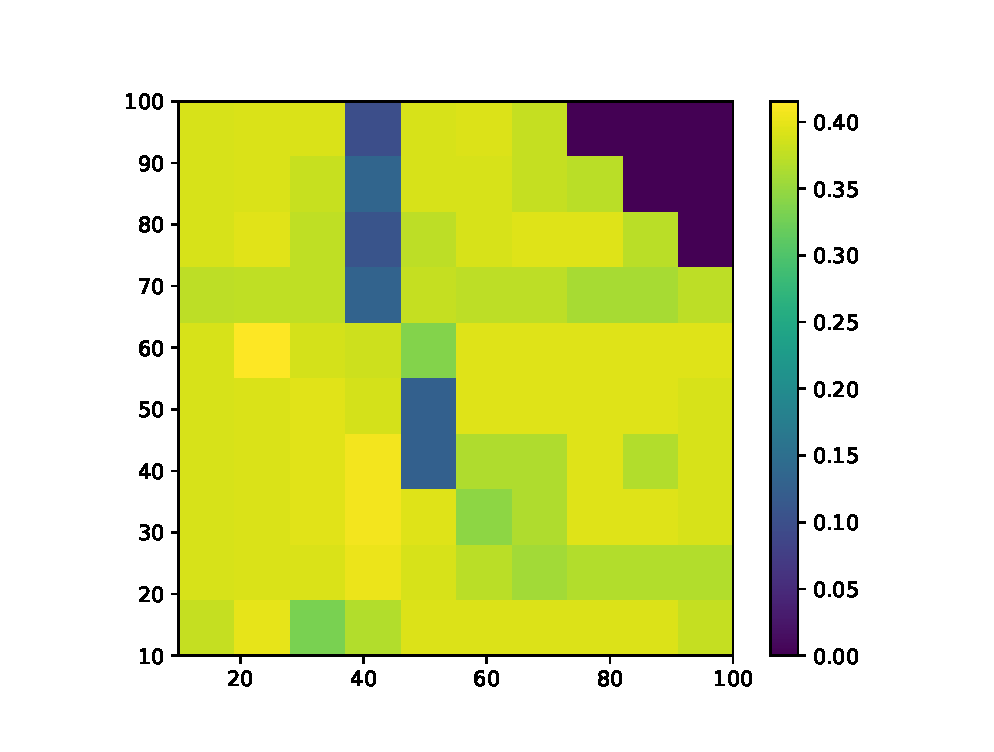
\includegraphics[width=0.5\columnwidth]{wine-lgm-colmap.eps}}
      \caption{\label{fig:iriskheatmap} Values of $k^+$ and $k^-$ vs. LGM accuracy. }
  \end{figure}
  For the iris dataset, where obtain satisfying results (around 80\%), there 
  exists a correlation between the parameters. The same doesn't hold for the 
  wine dataset. \\ 
    Secondly, a possible question we can ask is whether having dissimilarity 
  metrics (i.e. the edges relating farthest neighbours) actually improves the 
  accuracy. To this end, I also include the calculation of standard spectral 
  clustering using the laplacian, by only including $k$ neighbours.
    Bellow, I present a table of the best results obtained by each of these 
  algorithms for this dataset. The values are optimised by performing a grid search
  on possible values for $k_+$ and $k_-$.

  %insert table here%
  \begin{table}[h!]
    \centering
    \begin{tabular}{| l | l | l | l | l | l | }
      \hline
      dataset(classes) & LSym & LSN & LBN & LAM & LGM \\
      \hline
      wine(3) & 0.786  &  \textbf{0.818}  &  \textbf{0.818}  &  0.814  &  \textbf{0.818} \\   
      iris(3) & 0.433  &  \textbf{0.448}  &  \textbf{0.448}  &  0.444  &  0.415 \\
      digits(10) & \textbf{0.805}  &  0.728  &  0.729  &  0.705  &  0.762\\
      breast cancer(2) & 0.635  &  0.670  &  0.670  &  \textbf{0.676}  &  0.534 \\
      ecoli(4) & 0.751  &  0.679  &  0.679  &  \textbf{0.778}  &  0.694 \\
      \hline
    \end{tabular}
    \caption{ARI for Datasets in scikit-learn toy examples (wine, iris, digits, 
    and breast cancer) as well as URI(ecoli)}
  \end{table}

    We can compare these tables to graphs in the original paper. However, a conclusive 
  comparison cannot be conducted because \emph{Mercado et al.} do not specify,
  to the best of my knowledge, specifics of their clustering error calculations.
  On these datasets, the papers report the ratio of times when a certain method 
  was better or strictly better than the other, treating each selection of $k$ 
  as a separate problem. However, we treated the $k$s as hyperparameters to the 
  machine learning model, and reported the best result via grid search. 
    If instead we performed the original papers' analysis, we obtain slightly
  different results, we a favourable bias for the method that discards the 
  farthest neighbour. This suggests that maybe, the authors used a differnt metric
  for finding the k nearest (farthest) neighbours.
  
  \begin{table}[h!]
    \centering
    \begin{tabular}{| l | l | l | l | l | l | }
      \hline
      dataset / method & LSym & LSN & LBN & LAM & LGM  \\ 
      \hline
      wine &  \textbf{0.304}  &  0.240  &  0.144  &  0.141  &  0.171 \\   
      iris &  0.247  &  0.179  &  0.130  &  0.140  &  \textbf{0.305} \\
      digits & \textbf{0.357}  &  0.107  &  0.143  &  0.143  &  0.250\\
      breast cancer & \textbf{0.379}  &  0.207  &  0.103  &  0.276  &  0.034\\
      ecoli &  \textbf{0.407}  &  0.139  &  0.074  &  0.231  &  0.148\\
      \hline
    \end{tabular}
    \caption{Ratio of highest score during the grid search operation}
  \end{table}



  %caption of %



  \subsection{SNAP datasets}
  The paper suggests that the LGM method has, for the first time, found community 
  structure in the wikipedia data. Unfortunately, I have not been able to replicate
  this result. 
  However, I have been able to output results in the bitcoin-otc and bitcoin-alpha
  data. \cite{kumar2016edge}.
  One problem with analysing graph data in this format is the presence of
  disconnected components. If there are disconnected components in either of the 
  two matrices, $W^+$ or $W^-$, then their degree matrices will be singular. 
  This breaks the computation tree by disabling computing the inverse. 
  
  An initial solution I applied to alleviate this problem is to recursively remove 
  all the null rows and columns in the matrices. This makes sense in the current
  context since we are only interested in finding communities in connected 
  components. I have not analysed the optimality of this method (whether the 
  final matrix will have a maximal size), but it yielded good results. 

  Bellow, I present the $W^+$ and $W^-$ matrices for the two datasets, sorted after 
  the LGM clustering.

  \begin{figure}[h!]
    \centering
      \subfloat[$W^+$]{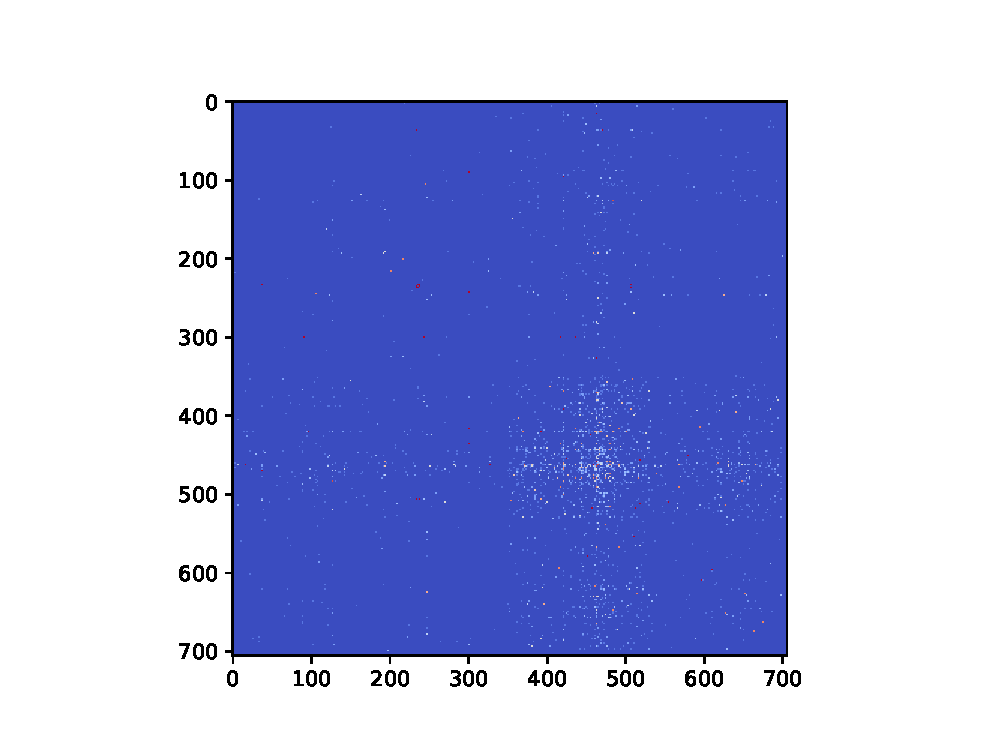
\includegraphics[width=0.5\columnwidth]{bitcoin-alpha-plus.eps}}
      \hfill
      \subfloat[$W^-$]{\includegraphics[width=0.5\columnwidth]{bitcoin-alpha-minus.eps}}
      \caption{\label{fig:bitcoinalphamap} Clustering on the Bitcoin-Alpha-Dataset \cite{kumar2016edge}.}
  \end{figure}

  \begin{figure}[h!]
    \centering
      \subfloat[$W^+$]{\includegraphics[width=0.5\columnwidth]{bitcoin-otc-plus.eps}}
      \hfill
      \subfloat[$W^-$]{\includegraphics[width=0.5\columnwidth]{bitcoin-otc-minus.eps}}
      \caption{\label{fig:bitcoinotcmap} Clustering on the Bitcoin-OTC-Dataset \cite{kumar2016edge}.}
  \end{figure}
  % show matrix plots %

  Although the data is very sparse, communities can be clearly identified in the $W^+$. Unfortunately,
  I have not been able to reproduce heatmaps similar to those present in the paper.

\section{Conclusion}

  \emph{Mercado et al.} \cite{mercado2016clustering} propose a new method for 
  performing spectral clustering on signed graph. They address the problem of 
  comparing to previous methods in a theoretical manner, and argue that the 
  spectral clustering using LGM should perform better on more graphs than the others.
  Furthermore, they manage to overcome the challenge posed by an expensive 
  eigenvalue decomposition by leveraging optimisations from properties of the 
  geometric mean. \\
  In the current work, I have tried to replicate their results and expand on 
  some evaluation techniques. 
  Firstly, I have tried to analyse the performance of clustering algorithms on the 
  SBM in Section \ref{ev:sbm}. In most of my tests, the LGM method yielded better
  results on SBM parametrized according to the axioms from table \ref{tab:ineq}.
  Very bipolar outcome result from all the clustering methods, showing that the 
  SBM method is not guaranteed to create communities. \\
  Next, I analysed the standard datasets in section \ref{ev:std}. Additionally to 
  the methods used previously, I have also tried to compare signed graph clustering
  to unsigned graph clustering. Unfortunately, the latter resulted in better
  accuracy than any of the signed methods. The LGM method seems to perform
  neither better nor worse compared to the other signed methods. However, my results
  are not conclusive, since I was very limited by the high computational cost (see 
  figure \ref{fig:increasingn}). I have also shown results of the grid search
  for the hyperparameters $k^+$ and $k^-$, which signal yet again that graph
  clustering tends to be, in general, limited by the vast differences between 
  graph structures. \\
   
  Finally, I have tried to apply the method on a signed graph dataset, to this end
  choosing the Bitcoin Otc and Alpha datasets \cite{kumar2016edge}. Although less 
  clear than similar figures presented by \emph{Mercado et al.}, communities have 
  certainly been detected. \\

\bibliography{mybib.bib}
\bibliographystyle{plain}
\end{document}
